
\begin{figure}
  \centering \includegraphics[width=0.66\textwidth]{./figs/bubble_figs/rt_linear}
  \caption{History of the bubble radius (top) and input-pressure
    waveform (bottom) for an essentially linear case (frequency: 1.5 MHz; peak y
    negative pressure: 0.35 MPa). No bioeffects are observed
    here. $R_0=1$ $\mu$m; solid: $G=5$ kPa; dashed: $G=100$ kPa; dotted: $G=1$ MPa.}
  \label{figure:sample_bubble_linear}
\end{figure}

\begin{figure}
  \centering 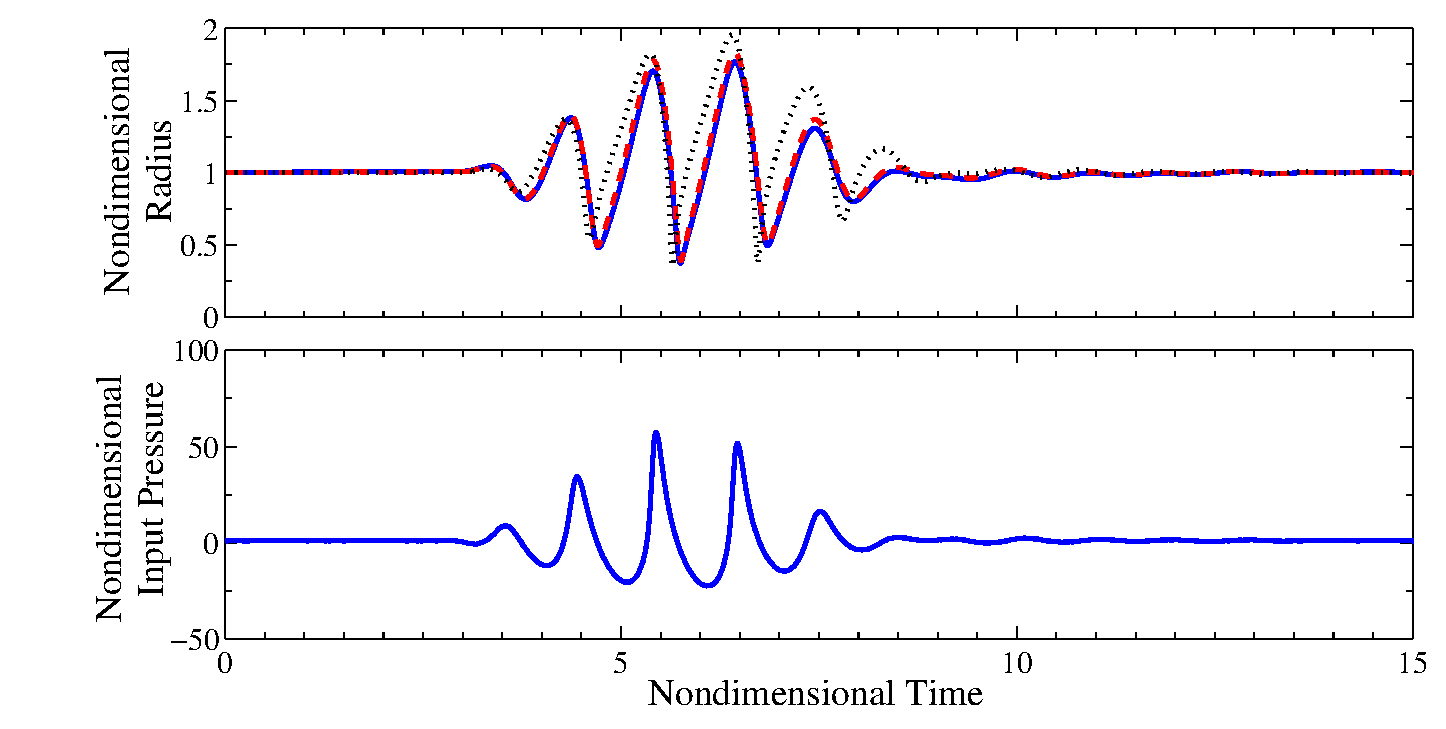
\includegraphics[width=0.66\textwidth]{./figs/bubble_figs/rt_intermediate}%
  \caption{History of the bubble radius (top) and input-pressure
    waveform (bottom) for a moderately nonlinear case (frequency: 3.5 MHz; peak 
    negative pressure: 2.4 MPa). Bioeffects are
    observed here. $R_0=1$ $\mu$m; solid: $G=5$ kPa; dashed: $G=100$ kPa;
    dotted: $G=1$ MPa.}
  \label{figure:sample_bubble_intermediate}
\end{figure}

\begin{figure}
  \centering \includegraphics[width=0.66\textwidth]{./figs/bubble_figs/rt_nonlinear}
  \caption{History of the bubble radius (top) and input-pressure
    waveform (bottom) for a highly nonlinear case (frequency: 
    7.5 MHz; peak negative pressure: 6.0 MPa). Bioeffects are observed
    here. $R_0=1$ $\mu$m; solid: $G=5$ kPa; dashed: $G=100$ kPa; dotted: $G=1$ MPa.}
  \label{figure:sample_bubble_nonlinear}
\end{figure}

In the results of the following sections, the maximum dimensionless radius,
$R_{max}$, and dimensional bubble temperature at collapse, $T_{max}$, obtained
using the ideal gas law, are determined by recording their largest
value over the simulation. These quantities are compared to the
inertial cavitation thresholds used by \cite{Apfel1991} and
\cite{Yang2005}: $R_{max}=2$ and $T_{max}=5000$ K. The dependence
of the bubble dynamics on the pulse amplitude, initial
bubble size (\emph{i.e.}, UCA size distribution), 
pulse frequency, and tissue properties are considered
individually. 



\subsection{Dependence on the Pulse Amplitude}

Given the strong dependence of the MI on the rarefactional pressure
amplitude, the influence of the pulse amplitude on the bubble dynamics
is first evaluated. Fig.~\ref{figure:amplitude} shows the dimensionless
maximum radius as a function of rarefactional pressure
amplitude. Initial bubble radii ranging between 0.1--2.0 $\mu$m are
shown, as well as different frequencies. The open symbols denote
cases where bioeffects did not occur, while the filled symbols denote
the occurrence of bioeffects.

\begin{figure}[t]
  \includegraphics[width=\columnwidth]{./figs/bubble_figs/rstarmax_pm}
  \caption{(color online) Dependence of the dimensionless maximum bubble radius on
    the peak negative pressure for $G=100$ kPa.  Empty symbols: no
    bioeffects; filled symbols: bioeffects. Pentagrams: 0.1 $\mu$m; circles:
    0.5 $\mu$m; squares: 1 $\mu$m; diamonds: 2 $\mu$m; frequency: 1.5 - 7.5 MHz. }
  \label{figure:amplitude}
\end{figure}

The results show that the bubble dynamics, through the maximum radius,
scale with the pulse amplitude. Although the results do not collapse fully
onto a line, a general trend is discernible. At low amplitude, the increase in
the maximum radius is approximately linear; beyond some amplitude, the bubble undergoes
nonlinear oscillations, thus explaining the different depenced and larger spread. 
These results are consistent with the plots shown in 
Figs.~\ref{figure:sample_bubble_linear}-\ref{figure:sample_bubble_nonlinear}.
Over a broad range of amplitudes, the
occurrence of bioeffects has little correlation with pulse amplitude
alone: at a given amplitude, bioeffects may be observed or not,
depending on the bubble size and pulse frequency.  Only at very large
pressure amplitudes (PRPA $>$ 4.20 MPa) are bioeffects systematically observed regardless of the
bubble size and pulse frequency. This behavior is not surprising, since at
these amplitudes the bubble response is expected to be highly
nonlinear. Conversely, at low amplitudes (PRPA $<$ 0.97 MPa), the oscillations are 
linear and no bioeffects are observed, regardless of
bubble size and pulse frequency. In this latter case, most bubbles
whose $R_{max}/R_o$ is below two do not exhibit bioeffects; however,
this behavior depends on the value of elasticity, as shown in \S
\ref{section:tissue_properties}.  Although not shown here for conciseness,
similar results are obtained for peak positive pressure.


Similarly, the criterion $T_{max} > 5000$ K is not achieved with perfluoropropane.
As shown in Fig.~\ref{figure:gascontents}, the observed temperatures for
PFP are far below this value, though the results for air approach it. This
result is expected since the criterion was determined for air, which
has a larger specific heats ratio ($\gamma_{air}=1.4$) than
PFP ($\gamma= 1.13$). The specific heats ratio appears in
the internal gas pressure term in Eq.~\ref{eq:bubble_pressure}; its
effect on the bubble dynamics is minor if the minimum radius is not
very small, as in Fig.~\ref{figure:gascontents}. Still, since the
adiabatic relationships for an ideal gas are used, the temperature is
significantly affected by the different specific heats ratio. Hence,
even though the bubble dynamics are not strongly affected by the
specific heats ratio, the maximum temperature is.

\begin{figure*}[t]
  \begin{subfigure}[b]{0.47\textwidth}
  \includegraphics[width=\textwidth]{./figs/bubble_figs/pfpair}
  \caption{History of the bubble radius for PFP (solid) and air
    (dashed). $R_0=1$ $\mu$m; frequency: 3.5 MHz; peak negative
    pressure: 3.3 MPa}
\end{subfigure}
  \begin{subfigure}[b]{0.47\textwidth}
    \includegraphics[width=\textwidth]{./figs/bubble_figs/tmaxpfpair} 
    \caption{Maximum temperature for PFP (circles) and air (squares). $R_0=0.1-2$ $\mu$m; frequency: 1.5 - 7.5 MHz.}
  \end{subfigure}
  \caption{(color online) Dependence of the bubble dynamics on the gas contents ($G=100$ kPa).}
  \label{figure:gascontents}
\end{figure*}

% \begin{figure*}[t]
%   \subfigure[History of the bubble radius for PFP (solid) 
%     and air (dashed). $R_0=1$ $\mu$m; frequency: 3.5 MHz; peak negative pressure: 3.3 MPa]{
%   \includegraphics[width=0.47\textwidth]{./figs/bubble_figs/pfpair} }
%   \subfigure[Maximum temperature for PFP (circles) and air (squares). $R_0=0.1-2$ $\mu$m; frequency: 1.5 - 7.5 MHz. ]{
%   \includegraphics[width=0.47\textwidth]{./figs/bubble_figs/tmaxpfpair} }
%   \caption{(color online) Dependence of the bubble dynamics on the gas contents
%   ($G=100$ kPa).}
%   \label{figure:gascontents}
% \end{figure*}






\subsection{Dependence on the Initial (Equilibrium) Bubble Radius}

In the experiment, the size distribution of the UCAs is not known
exactly. It is desirable to know whether the observed bioeffects are
caused by all bubbles responding to the ultrasound, or whether a
specific size is more likely to be responsible at the bioeffects
threshold. To answer this question, for each experimental frequency,
bubbles of different radii ranging from 0.1--2 $\mu$m are subjected to
the pressure waveform corresponding to the bioeffects threshold
amplitude. It should be noted that varying the equilibrium radius
changes the non-dimensional parameters. Fig.~\ref{figure:size} shows the maximum dimensionless
radius, for both water (zero elasticity) and tissue (finite
elasticity, $G=100$ kPa), for the amplitude at which bioeffects are
first observed at a given frequency.

\begin{figure}[t]
    \includegraphics[width=\columnwidth]{./figs/bubble_figs/rstarmax_r0}
    \caption{(color online) Dependence of the dimensionless maximum bubble radius on
      the initial bubble size for the amplitude at which bioeffects
      are first observed, at a given frequency, for $G=100$ kPa. Empty
      symbols: water; filled symbols: tissue. Circles: 1.50 MHz; squares:
      2.25 MHz; diamonds: 3.50 MHz; pentagrams: 5.00 MHz; hexagrams: 7.50 MHz.}
    \label{figure:size}
\end{figure}

Excluding the smallest size, the bubble response in tissue is monotone
and changes little for a given frequency; there is no initial size
that consistently leads to a dramatic response. The somewhat erratic
behavior of the small bubbles may imply that such sizes are not
present in UCA concentrations. On the other hand, the behavior is more
irregular for water, particularly at small radii: for a given
frequency, there is an optimal size that exhibits the largest
response; these variations are much larger than for tissue.  








\subsection{Dependence on the Pulse Frequency}

The dependence of the bubble response on the pulse frequency is
considered in this section.  Fig.~\ref{figure:freq} shows the maximum
dimensionless and dimensional radius for all initial bubble sizes and
amplitudes vs. frequency. The square symbols denote cases in which
bioeffects were observed in the experiments, while the circular symbols
represent no bioeffects. The initial bubble sizes are not
discriminated here for simplicity.


\begin{figure*}[t]
  \begin{subfigure}[b]{0.47\textwidth}
    \includegraphics[width=\textwidth]{./figs/bubble_figs/rstarmax_f}  
    \caption{Dimensionless maximum bubble radius.}
  \end{subfigure}

  \begin{subfigure}[b]{0.47\textwidth}
    \includegraphics[width=0.47\textwidth]{./figs/bubble_figs/rmax_f}      
    \caption{Dimensional maximum bubble radius.}
  \end{subfigure}
  \caption{(color online) Dependence of the bubble dynamics on the frequency for
    $G=100$ kPa. $R_0=0.1-2$ $\mu$m; empty circles: no bioeffects; squares:
    bioeffects.}
  \label{figure:freq}
\end{figure*}

With the exception of a few outliers, a clear separation between cases
for which bioeffects did and did not occur is observed; in other
words, the bioeffects threshold has a strong dependence on the
frequency. The trend appears to be approximately linear with
frequency. Large growth may be achieved with no evident bioeffects,
especially at high frequencies. The quantity $R_{max}$ is a
measure of cavitation collapse, since it is related to the available
energy of the bubble. Thus, the present results indicate that
cavitation collapse is expected to play an important role regarding
bioeffects, although the precise mechanism cannot be inferred.  Again,
the existing criteria for inertial cavitation thresholds are
frequency-independent and do not correlate well with the bioeffects
threshold, which clearly shows a strong dependence on frequency.

Another hypothesis is that bubble growth may be responsible for
capillary breaching. However, the plot of the dimensional maximum radius vs. frequency does
not show systematic bioeffects beyond a certain size, \emph{e.g.},
some capillary diameter. Thus, growth is not the sole mechanism by
which bioeffects occur. However, the data remains inconclusive,
due to the inability to identify the cases in which cavitation
collapse is the dominant effect.






\subsection{Dependence on the Tissue Properties}
\label{section:tissue_properties}

As suggested in
Figs.~\ref{figure:sample_bubble_linear}-\ref{figure:sample_bubble_nonlinear},
the bubble dynamics are sensitive to the tissue properties,
specifically the elasticity. However, different types of tissue may
have very different properties. Many of the measurements of tissue elasticity are made
\emph{in vitro}, and depend strongly on tissue preparation, storage,
and degradation as well as method of measurement.  Consequently it is
possible that these measurements do not accurately represent the
current behavior.  To explore the effect of the elasticity on the
results and the correlation to bioeffects, Fig.~\ref{figure:freq_tissue}
shows the maximum dimensionless radius for all initial bubble sizes
and amplitudes vs. frequency for $G=5$ kPa and $G=1$ MPa. Although
seemingly high, the latter elasticity is chosen to match the work of
\cite{Yang2005}.

\begin{figure*}[t]
  \begin{subfigure}[b]{0.47\textwidth}
    \includegraphics[width=\textwidth]{./figs/bubble_figs/rstarmax_f_ca=20}
    \caption{$G=5$ kPa.}
  \end{subfigure}

  \begin{subfigure}[b]{0.47\textwidth}
    \includegraphics[width=\textwidth]{./figs/bubble_figs/rstarmax_f_ca=0,1}    
    \caption{$G=1$ MPa.}
  \end{subfigure}
  \caption{(color online) Dependence of the dimensionless maximum bubble radius on
     the frequency. $R_0=0.1-2$ $\mu$m; empty circles: no bioeffects; squares:
     bioeffects.}
  \label{figure:freq_tissue}
\end{figure*}

% \begin{figure*}[t]
%   \subfigure[$G=5$ kPa.]{
%     \includegraphics[width=0.47\textwidth]{./figs/bubble_figs/rstarmax_f_ca=20}
%   }
%   \subfigure[$G=1$ MPa.]{
%     \includegraphics[width=0.47\textwidth]{./figs/bubble_figs/rstarmax_f_ca=0,1}    
%   }
%    \caption{(color online) Dependence of the dimensionless maximum bubble radius on
%      the frequency. $R_0=0.1-2$ $\mu$m; empty circles: no bioeffects; squares:
%      bioeffects.}
%   \label{figure:freq_tissue}
% \end{figure*}

The bubble dynamics and correlation to bioeffects significantly change
when reducing the elasticity. For a value of 5 kPa, the discrimination
is no longer clear. The bubble dynamics are closer to the behavior in
water, such that different sizes may have dramatically different
responses to the same waveform, as explained previously. On the other
hand, the stiffer medium ($G=1$ MPa) shows an even sharper
demarcation, which again appears to be approximately linear. Given the
sensitivity of the results on the elasticity, it is clear that more
precise \emph{in vivo} data is required for elasticities of tissues at the
relevant strain rates. 

Although not shown here, the type of
viscoelastic model significantly affects the bubble dynamics
\cite[]{Johnsen2012}. For instance, a standard linear solid
model, which includes stress relaxation in addition to elasticity, leads 
to very different maximum
radii and oscillation properties (frequency and damping).  For
large relaxation times, elasticity variations become negligible.




\section{Conclusions}
\label{sec:usbe_bubble_conclusions}

In the present work, a numerical model is used
to investigate experimentally observed bioeffects as a result of
contrast-enhanced ultrasound. This work is unique in its 
combination of experimental results and numerical modeling.
For the experimentally generated input
pressure waveforms, it is known which of these triggered bioeffects,
and from the numerical model we obtained calculated values for
the dimensionless maximum radius and dimensional maximum temperature for each of these cases.  By comparing the
results of this study to previously established inertial cavitation
thresholds used by \cite{Apfel1991} and \cite{Yang2005},
$T_{max}=5000$ K and $R_{max}=2$, it would appear that the inertial
cavitation threshold does not play a role in determining the bioeffects
threshold.  However, it is unlikely that the inertial cavitation
threshold is irrelevant. Instead, it is far more probable that these
thresholds are not defined appropriately for cavitation in a
viscoelastic medium, such as soft tissue. This work suggests the need for
further experimental and numerical studies of cavitation in viscoelastic media.

The present work shows a strong correlation between cavitation dynamics and bioeffects
when considering the pulse frequency.
From the plot of maximum
dimensionless radius vs. frequency, there is a clear separation
between when bioeffects do and do not occur, and based on these
results it appears that the frequency of the input pressure waveforms
is of key importance to the definition of a bioeffect threshold, and
likely the inertial cavitation threshold as well. 

The present work shows that the elasticity of tissue significantly
affects the bubble dynamics. This finding is perhaps not completely
unexpected given that bubble dynamics are known to strongly depend
on viscoelastic properties and model. The present study shows the need
for more accurate measurements of material properties and for
determining appropriate constitutive models for soft tissue,
particularly at high strain rates. Finally, although the present work
suggests that inertial cavitation collapse plays an important role with respect
to bioeffects, it does not shed light on the exact mechanism,
\emph{e.g.}, shock emission upon collapse, growth beyond a given size,
high temperatures generating free radicals, re-entrant jets in
non-spherical collapse, etc.  In future work we plan on investigating 
this injury mechanism by conducting direct simulations of
the full equations of motion for bubble dynamics in a viscoelastic medium.


%%% Local Variables:
%%% mode: latex
%%% TeX-master: t
%%% End:
